\documentclass[12pt, oneside]{article}
\usepackage[letterpaper, margin=1in, headsep=0.5in, left=0.3in, right=2.5in]{geometry}
\usepackage[english]{babel}
\usepackage[utf8]{inputenc}
\usepackage{amsmath}
\usepackage{amsfonts}
\usepackage{amssymb}
\usepackage{tikz}
\usepackage{yhmath}
\usetikzlibrary{quotes, angles}
\usepackage{graphicx}
\usepackage{enumitem}
\usepackage{multicol}

\newif\ifmeta
\metatrue %print standards and topics tags

\title{Regents Geometry}
\author{Chris Huson}
\date{May 2022}

\usepackage{fancyhdr}
\pagestyle{fancy}
\fancyhf{}
\renewcommand{\headrulewidth}{0pt} % disable the underline of the header
\raggedbottom

%\fancyhead[LE]{\thepage}
\fancyhead[RO]{Name:}
\fancyhead[LO]{BECA / Dr. Huson / Geometry Regents Mixed Review}
\cfoot{\thepage}

\begin{document}
\subsubsection*{11.17 Rotation plus dilation}
\begin{enumerate}[itemsep=1.2cm]
\item Given $\triangle ABP \sim \triangle JKP$ as shown below. $AB=12.5$, $AP=13.5$, $BP=7.1$, and $JP=32.4$. Find $JK$.
    \begin{flushright}
    \begin{tikzpicture}[scale=1.4]
        \draw [thick]
          (-0.25,-1)node[below left]{$B$}--
          (0.5,2)node[left]{$K$}--
          (4,0)node[below left]{$J$}--
          (0,0)node[above left]{$P$}--
          (-2,0)node[left]{$A$}--cycle;
      \end{tikzpicture}
      \end{flushright}

\item Write an equation of the line that is parallel to the line whose equation is $4y+8=3x$ and passes through the point $(1,-3)$.

\item The base of a pyramid is a rectangle with a width of 11.2 cm and a length of 8.5 cm. What is the height, in centimeters, of the pyramid if its volume is 238 cm$^3$?

\item In the diagram below of right triangle $ABC$, $AC=8$, and $AB=10$.
  \begin{center}
    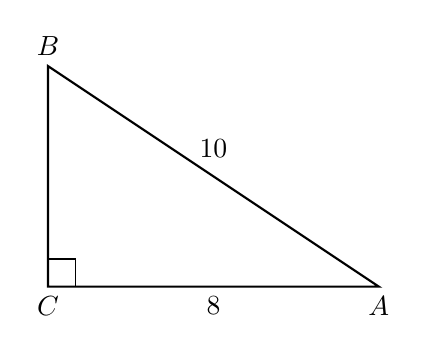
\begin{tikzpicture}[scale=0.7]
    \draw [thick]
      (0,0)node[below]{$A$}--
      (-6,4)node[above]{$B$}--
      (-6,0)node[below]{$C$}--cycle;
      \draw (-6,0)++(0.5,0)--++(0,0.5)--+(-0.5,0);
      \node at (-3,0)[below]{$8$};
      \node at (-3,2.5){$10$};
  \end{tikzpicture}
  \end{center}
    Which equation would determine the value of angle $A$?
  \begin{multicols}{2}
    \begin{enumerate}
      \item $\displaystyle \sin A = \frac{8}{10}$
      \item $\displaystyle \tan A = \frac{8}{6}$
      \item $\displaystyle \cos A = \frac{6}{10}$
      \item $\displaystyle \tan A = \frac{6}{8}$
    \end{enumerate}
  \end{multicols}

\newpage

\item What is the equation of a circle with center $(4,-2)$ and radius $r=5$?

\item In a right triangle, the acute angles have the relationship \\$\sin (3x + 4)=\cos (37)$.\\[0.25cm]
    What is the value of $x$?

\item In the diagram below of right triangle $KMI$, altitude $\overline{IG}$ is drawn to hypotenuse $\overline{KM}$.
\begin{center}
  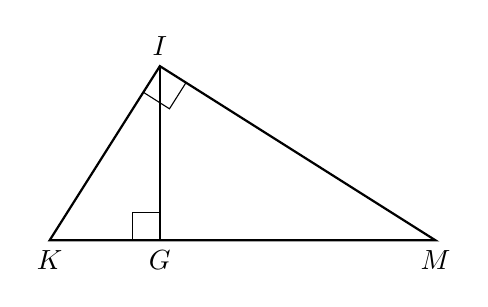
\begin{tikzpicture}[scale=0.7]
  \draw [thick]
  (0,0)node[below]{$K$}--
  (7,0)node[below]{$M$}--
  (2,3.16)node[above]{$I$}--cycle;
  \draw (2,3.16)++(-0.15*2,-0.15*3.16)--++(0.15*3.16,-0.15*2)--+(0.15*2,0.15*3.16);
  \draw [thick](2,0)node[below]{$G$}--(2,3.16);
  \draw (2,0)++(-0.5,0)--++(0,0.5)--+(0.5,0);
\end{tikzpicture}
\end{center}
IF $KG=4$ and $IG=6$, what is the length of $\overline{IM}$?
\vspace{2cm}

\item Circle $O$ has chords $\overline{AD}$ and $\overline{BE}$ intersecting at $C$, as shown. Find $AC$.
\begin{center}
  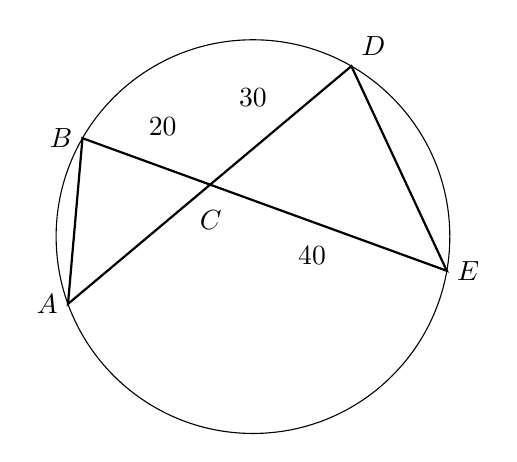
\begin{tikzpicture}[scale=0.5]
   \draw (0,0) circle[radius=5];
   \draw [thick]
   (-10:5) node[right] {$E$}--
   (150:5) node[left] {$B$}--
   (200:5) node[left] {$A$}--
   (60:5) node[above right] {$D$}--cycle;
   \draw (140:1.4) node[below] {$C$};
   \draw (125:4) node[below] {$20$};
   \draw (90:4) node[below] {$30$};
   \draw (0:1.5) node[below] {$40$};
  \end{tikzpicture}
\end{center}

\end{enumerate}
\end{document}
  